\section{MEG analysis \label{multimodal:data:meg}}

\subsection{Preprocessing the MEG data\label{multimodal:data:meg:preproc}}

First change directory to the MEG subdirectory (either in \matlab\, or via the ``CD'' option in the SPM ``Utils'' menu)

\subsection{Adjust trigger latency}

For the EEG data, the faces were displayed directly via a CRT monitor. For the MEG data on the other hand, the faces were displayed inside the MSR via a projector. This projector produces a delay of 1.5 screen refreshes, which at 60Hz, is 25ms. This means that the subject actually saw the stimuli 25ms after the trigger was sent to the MEG acquisition machine. To correct for this visual delay, we will illustrate how to manipulate ``trial'' structures\footnote{Alternatively, you could correct by 1 refresh, to match the delay in the EEG data.}. First, we need to read in the triggers from the MEG data (unlike the EEG dataset, the MEG dataset contains information about trial type so we can define the correct condition labels already at this stage). To do this, type the following in the \matlab\ window:

\begin{verbatim}
    [trl, conditionlabels, S] = spm_eeg_definetrial;
\end{verbatim}

and follow these steps:
\begin{itemize}
 \item Select the \texttt{SPM\_CTF\_MEG\_example\_faces1\_3D.ds/SPM\_CTF\_MEG\_example\_faces1\_3D.meg4} file.
 \item Enter \texttt{-200} for ``Start of trial in PST [ms]'' and \texttt{600} to ``End of trial in PST [ms]''.
 \item Enter 2 for ``How many conditions?''.
 \begin{itemize}
  \item Enter ``\texttt{faces}'' for ``Label of condition 1''. A dialog with a list of events will come up and Select the event with type \texttt{UPPT001\_up} and Value 1.
  \item Enter ``\texttt{scrambled}'' for ``Label of condition 2''. Select the even with type \texttt{UPPT001\_up} and Value 2.
 \end{itemize}
 \item Answer ``no'' to the question about reviewing trials.
 \item Answer ``yes'' to the prompt to save the trial definition.
 \item Enter a filename like \texttt{trials\_run1.mat} and save in the MEG directory.
\end{itemize}

Then type \texttt{load trials\_run1.mat} in \matlab\, to see the contents of the file you just saved. It contains two variables, \texttt{trl} and \texttt{conditionlabels}. The \texttt{trl} variable contains as many rows as triggers were found (across all conditions) and three columns: the initial sample of the epoch, the final sample of the epoch and the offset in samples corresponding to a peristimulus time of 0. The sampling rate for the MEG data was 480Hz (as can be found in the \texttt{S.fsample} field of the structure \texttt{S} returned by the \texttt{spm\_eeg\_definetrial} call above). Thus the figure of -96 samples in the third column corresponds to the 200ms baseline period that you specified. Now we need to shift the initial and final samples of the epochs by 25ms. You can do this by typing:

\begin{verbatim}
    trl(:,1:2) = trl(:,1:2) + round(25*S.fsample/1000);
    save trials_run1 trl conditionlabels
\end{verbatim}

The new trial definition is thus resaved, and we can use this file when next converting the data.

\subsection{Convert}

Press the \textsc{Convert} button, and in the file selection window again select the \texttt{SPM\_CTF\_MEG\_example\_\-faces1\_3D.ds} subdirectory and the \texttt{\hyphenchar\font45\relax SPM\_CTF\_MEG\_example\_faces1\_3D.meg4} file. At the prompt ``Define settings?'' select ``yes''. Here we will use the option to define more precisely the part of data that should be read during conversion. Answer ``trials'' to ``How to read?'', and ``file'' to ``Where to look for trials?''. Then in the file selector window, select the new \texttt{trials\_run1.mat} file. Press ``no'' to ``Read across trials?'' and select ``meg'' for ``What channels?''. Press ``no'' to avoid saving the channel selection. Press ``Enter'' to accept the default suggestion for the name of the output dataset. Two files will be generated \texttt{espm8\_SPM\_CTF\_MEG\_example\_faces1\_3D.mat} and \texttt{espm8\_SPM\_CTF\_MEG\_example\_faces1\_3D.dat}. After the conversion is complete the data file will be automatically opened in the SPM8 reviewing tool. If you click on the ``MEG'' tab you will see the MEG data which is already epoched. By pressing the ``intensity rescaling'' button (with arrows pointing up and down) several times you will start seeing MEG activity.

\subsection{Baseline correction}

We need to perform baseline correction as it is not done automatically during conversion. This will prevent excessive edge artefacts from appearing after subsequent filtering and downsampling. Select \textsc{Baseline correction} from the ``Other'' drop-down menu and select the \texttt{espm8\_SPM\_CTF\_MEG\_example\_faces1\_3D.mat} file. Enter $[-200\: 0]$ for ``Start and stop of baseline [ms]''. The progress bar will appear and the resulting data will be saved to dataset \texttt{bespm8\_SPM\_\-CTF\_\-MEG\_\-example\_faces1\_3D.\{mat,dat\}}.

\subsection{Downsample}

Select \textsc{Downsample} from the ``Other'' drop-down menu and select the \texttt{bespm8\_SPM\_CTF\_\-MEG\_\-example\_\-faces1\_3D.mat} file. Choose a new sampling rate of 200 (Hz). The progress bar will appear and the resulting data will be saved to dataset \texttt{dbespm8\_SPM\_CTF\_MEG\_example\_faces1\_3D.\{mat,dat\}}.

\subsection{Batch preprocessing}

Here we will preprocess the second half of the MEG data using using the SPM8 batch facility to demonstrate this third (after interactive GUI and Matlab script) possibility. First though, we have to correct the visual onset latency for the second run, repeating the above steps that you did for the first run:

\begin{verbatim}
    [trl, conditionlabels, S] = spm_eeg_definetrial;
\end{verbatim}

and select the \texttt{SPM\_CTF\_MEG\_example\_faces2\_3D.ds} subdirectory and the \texttt{SPM\_\-CTF\_\-MEG\_\-example\_\-faces2\_3D.meg4} file. Then enter \texttt{-200} for ``Start of trial in PST [ms]'' and \texttt{600} to ``End of trial in PST [ms]''. Enter \texttt{2} for ``How many conditions?''. Enter ``\texttt{faces}'' for ``Label of condition 1''. A dialog with a list of events will come up. Select the event with type ``\texttt{UPPT001\_up}'' and Value 1. Enter \texttt{scrambled} for ``Label of condition 2''. Select the event with type ``\texttt{UPPT001\_up}'' and Value 2. Answer ``no'' to the question about reviewing trials, but ``yes'' to the prompt to save the trial definition. Enter a filename like \texttt{trials\_run2.mat} and save in the MEG directory. Then type:

\begin{verbatim}
    load trials_run2
    trl(:,1:2) = trl(:,1:2)+round(25*S.fsample/1000);
    save trials_run2 trl conditionlabels
\end{verbatim}

Now press the \textsc{Batch} button (lower right corner of the SPM8 menu window). The batch tool window will appear. We will define exactly the same settings as we have just done using the interactive GUI. From the ``SPM'' menu, ``M/EEG'' submenu select ``M/EEG Conversion''. Click on ``File name'' and select the \texttt{SPM\_CTF\_MEG\_example\_faces2\_3D.meg4} file from \texttt{SPM\_CTF\_\-MEG\_\-example\_\-faces2\_3D.ds} subdirectory. Click on ``Reading mode'' and switch to ``Epoched''. Click on ``Epoched'' and choose ``Trial file'', double-click on the new ``Trial file'' branch and then select the \texttt{trials\_run2.mat} file.  Then click on ``Channel selection'' and select MEG from the menu below. Finally enter \texttt{espm8\_SPM\_CTF\_MEG\_example\_faces2\_3D} for ``Output filename'' to be consistent with the file preprocessed interactively.

Now select ``M/EEG Baseline correction'' from the ``SPM'' menu, ``M/EEG'' submenu. Another line will appear in the Module list on the left. Click on it. The baseline correction configuration branch will appear. Select ``File name'' with a single click. The file that we need to downsample has not been generated yet but we can use the ``Dependency'' button. A dialog will appear with a list of previous steps (in this case just the conversion) and we can set the output of one of these steps as the input to the present step. Now just enter enter $-200\: 0$ for ``Baseline''. Similarly we can now add ``M/EEG Downsampling'' to the module list, define the output of baseline correction step for ``File name'' and 200 for the ``New sampling rate''. This completes our batch. We can now save it for future use (e.g, as \texttt{batch\_meg\_preprocess} and run it by pressing the green ``Run'' button. This will generate all the intermediate datasets and finally \texttt{dbespm8\_SPM\_CTF\_MEG\_example\_faces2\_3D.\{mat,dat\}}.

\subsection{Merge}

We will now merge the two epoched files we have generated until now and continue working on the merged file. Select the \textsc{Merge} command from the ``Other'' drop-down menu. In the selection window that comes up click on \texttt{dbespm8\_SPM\_CTF\_MEG\_example\_faces1\_3D.mat} and \texttt{dbespm8\_SPM\_CTF\_MEG\_example\_faces2\_3D.mat}. Press ``done''. Answer ``Leave as they are'' to ``What to do with condition labels?''. A new dataset will be generated called \texttt{cdbespm8\_SPM\_CTF\_\-MEG\_\-example\_\-faces1\_\-3D.\{mat,dat\}}.

\subsection{Reading and preprocessing data using Fieldtrip}
Yet another even more flexible way to pre-process data in SPM8 is to use the Fieldtrip toolbox (\url{http://www.ru.nl/neuroimaging/fieldtrip/}) that is distributed with SPM. All the pre-processing steps we have done until now can also be done in Fieldtrip and the result can then be converted to SPM8 dataset. An example script for doing so can be found in the 
\texttt{man$\backslash$example\_scripts$\backslash$spm\_ft\_multimodal\_preprocessing.m}. The script will generate a merged dataset and save it under the name \texttt{ft\_SPM\_CTF\_\-MEG\_\-example\_\-faces1\_\-3D.\{mat,dat\}}. The rest of the analysis can then be done as below. This option is more suitable for expert users well familiar with Matlab. Note that in the script \texttt{ft\_} prefix is added to the names of all Fieldtrip functions. This is a way specific to SPM8 to call the functions from Fieldtrip version included in SPM distribution and located under \texttt{external$\backslash$fieldtrip}.

\subsection{Prepare}

In this section we will add the separately measured headshape points to our merged dataset. This is useful when one wants to improve the coregistration using head shape measured outside the MEG. Also in some cases the anatomical landmarks detectable on the MRI scan and actual locations of MEG locator coils do not coincide and need to be measured in one common coordinate system by an external digitizer (though this is not the case here). First let's examine the contents of the headshape file. If you load it into \matlab\ workspace (type \texttt{load headshape.mat}), you will see that it contains one \matlab\ structure called \texttt{shape} with the following fields:
\begin{itemize}
\item \texttt{.unit} - units of the measurement (optional)
\item \texttt{.pnt} - Nx3 matrix of headshape points
\item \texttt{.fid} - substruct with the fields .pnt - Kx3 matrix of points and .label -Kx1 cell array of point labels.
\end{itemize}

The difference between \texttt{shape.pnt} and \texttt{shape.fid.pnt} is that the former contains unnamed points (such as continuous headshape measurement) whereas the latter contains labeled points (such as fiducials). Note that this Polhemus space (which will define the ``head space'') has the X and Y axes switched relative to MNI space.

Now select \textsc{Prepare} from the ``Other'' menu and in the file selection window select \texttt{cdbespm8\_\-SPM\_\-CTF\_\-MEG\_\-example\_\-faces1\_3D.mat}. A menu will appear at the top of SPM interactive window (bottom left window). In the ``Sensors'' submenu choose ``Load MEG Fiducials/Headshape''. In the file selection window choose the \texttt{headshape.mat} file and save the dataset with \texttt{File/Save}.

If you do not have a separately measured headshape and are planning to use the original MEG fiducials for coregistration, this step is not necessary. As an exercise, you can skip it for the tutorial dataset and later do the coregistration without the headshape and see if it affects the results.

\subsection{Basic ERFs} 

Press the \textsc{Averaging} button and select the \texttt{cdbespm8\_SPM\_CTF\_MEG\_example\_faces1\_3D.mat} file. Answer ``yes'' to ``Use robust averaging?''. You can either save the weights if you want to examine them or not save if you want the averaging to work faster since the weights dataset that needs to be written is quite large. Answer ``no'' to ``weight by condition'' and accept the default ``Offset of the weighting function''. A new dataset will be created in the MEG directory called \texttt{mcdbespm8\_SPM\_CTF\_MEG\_example\_faces1\_3D.\{mat,dat\}} (``m'' for ``mean'').

As before, you can display these data by ``Display: M/EEG'' and selecting the \texttt{mcdbespm8\_\-SPM\_\-CTF\_\-MEG\_\-example\_\-faces1\_3D.mat}. In the MEG tag with the scalp radio button selected, hold the Shift key and select trial-type 2 with the mouse in the bottom right of the window to see both conditions superimposed (as Figure~\ref{multimodal:fig:10}).

\begin{figure}
\begin{center}
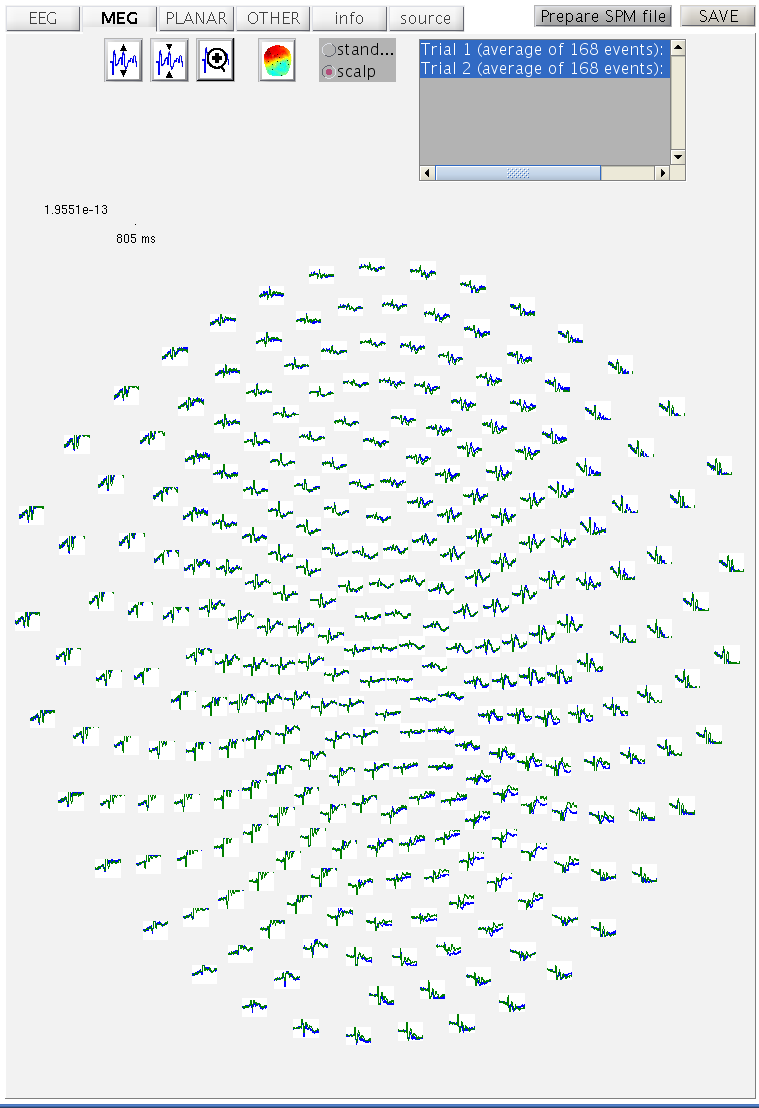
\includegraphics[width=100mm]{multimodal/figures/meg_scalp_erf}
\caption{\em SPM Display window for mean, smoothed ERF (\texttt{mcdbespm8\_\-SPM\_\-CTF\_\-MEG\_\-example\_\-faces1\_\-3D.mat}) for all 275 MEG channels. \label{multimodal:fig:10}}
\end{center}
\end{figure}

Select ``Contrast'' from the ``Other'' pulldown menu on the SPM window. This function creates linear contrasts of ERPs/ERFs. Select the \texttt{mcdbespm8\_SPM\_CTF\_MEG\_example\_faces1\_3D.mat} file, enter $[1\: -1]$ as the first contrast and label it ``\texttt{Difference}'', answer ``yes'' to ``Add another'',  enter $[1/2\: 1/2]$ as the second contrast and label it ``\texttt{Mean}''. Press ``no'' to the question ``Add another'' and not to ``weight by num replications''. This will create new file \texttt{wmcdbespm8\_\-SPM\_\-CTF\_\-MEG\_\-example\_\-faces1\_\-3D.mat}, in which the first trial-type is now the differential ERF between faces and scrambled faces, and the second trial-type is the average ERF for faces and scambled faces.

To see the topography of the differential ERF, select ``Display: M/EEG'', MEG tab and click on Trial 1, press the ``topography'' button at the top of the window and scroll to 180ms for the latency to produce Figure~\ref{multimodal:fig:12}.

You can move the slider left and right to see the development of the M170 over time.

\begin{figure}
\begin{center}
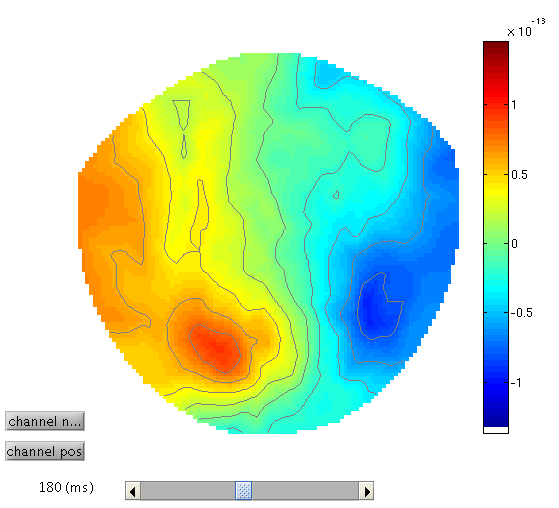
\includegraphics[width=100mm]{multimodal/figures/meg_topo180}
\caption{\em 2D topography of the ERF of faces minus scrambled faces at 180ms. \label{multimodal:fig:12}}
\end{center}
\end{figure}

\subsection{Time-Frequency Analysis}

SPM can use several methods for time-frequency decomposition. We will use Morlet wavelets for our analyses.

Select the \textsc{time-frequency} option under the ``Other'' pull-down menu. SPM batch tool with time-frequency configuration options will apear. Double-click on ``File name'' and select the \texttt{cdbespm8\_\-SPM\_\-CTF\_\-MEG\_\-example\_\-faces1\_\-3D.mat} file. Then click on ``Channel selection'' and in the box below click on ``Delete: All(1)'' and then on ``New: Custom channel''. Double-click on ``Custom channel'' and enter ``MLT34''.\footnote{You can of course obtain time-frequency plots for every channel, but it will take much longer (and result in a large file).} Double-click on ``Frequencies of interest'' and type [5:40] (Hz). Click on ``Spectral estimation'' and select ``Morlet wavelet transform''. Change the number of wavelet cycles from 7 to 5. This factor effectively trades off frequency vs time resolution, with a lower order giving higher temporal resolution. Select ``yes'' for ``Save phase?''.

This will produce two new datasets, \texttt{tf\_\-cdbespm8\_\-SPM\_\-CTF\_\-MEG\_\-example\_\-faces1\_3D.\{mat,dat\}} and  \texttt{tph\_\-cdbespm8\_\-SPM\_\-CTF\_\-MEG\_\-example\_\-faces1\_\-3D.\{mat,dat\}}. The former contains the power at each frequency, time and channel; the latter contains the corresponding phase angles.

Here we will not baseline correct the time-frequency data because for frequencies as low as 5Hz, one would need a longer pre-stimulus baseline, to avoid edge-effects\footnote{For example, for 5Hz, one would need at least N/2 x 1000ms/5, where N is the order of the Morlet wavelets (i.e, number of cycles per Gaussian window), e.g, 600ms for a 6th-order wavelet.}. Later, we will compare two trial-types directly, and hence any pre-stimulus differences will become apparent. 

Press the \textsc{Averaging} button and select the \texttt{tf\_\-cdbespm8\_\-SPM\_\-CTF\_\-MEG\_\-example\_\-faces1\_\-3D.mat} file. You can use straight (or robust if you prefer) averaging to compute the average time-frequency representation. A new file will be created in the MEG directory called \texttt{mtf\_cdbespm8\_\-SPM\_\-CTF\_\-MEG\_\-example\_\-faces1\_\-3D.\{mat,dat\}}. Note that you can use the reviewing tool to review the time-frequency datasets.

This contains the power spectrum averaged over all trials, and will include both ``evoked'' and ``induced'' power. Induced power is (high-frequency) power that is not phase-locked to the stimulus onset, which is therefore removed when averaging the amplitude of responses across trials (i.e, would be absent from a time-frequency analysis of the \texttt{mcdbespm8\_SPM\_\-CTF\_\-MEG\_\-example\_\-faces1\_\-3D.mat} file).

The power spectra for each trial-type can be displayed using the usual Display button and selecting the \texttt{mtf\_\-cdbespm8\_\-SPM\_\-CTF\_\-MEG\_\-example\_\-faces1\_3D.mat} file. This will produce a plot of power as a function of frequency (y-axis) and time (x-axis) for Channel MLT34. If you use the ``trial'' slider to switch between trial(types) 1 and 2, you will see the greater power around 150ms and 10Hz for faces than scrambled faces (click on the magnifying glass icon and on the single channel to get scales for the axes, as in Figure~\ref{multimodal:fig:13}). This corresponds to the M170 again.

\begin{figure}
\begin{center}
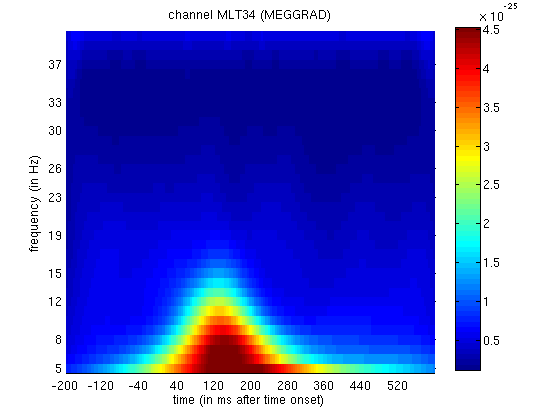
\includegraphics[width=60mm]{multimodal/figures/meg_pow_faces}
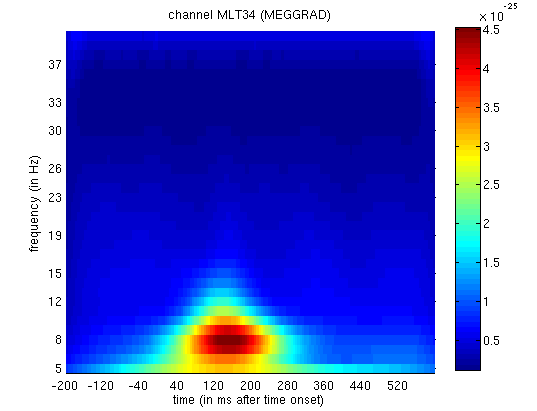
\includegraphics[width=60mm]{multimodal/figures/meg_pow_scrambled}
\caption{\em  Total power spectra for faces (left) and scrambled faces (right) for channel MLT34\label{multimodal:fig:13}}
\end{center}
\end{figure}

We can also look at evidence of phase-locking of ongoing oscillatory activity by averaging the phase angle information. We compute the vector mean (by converting the angles to vectors in Argand space), which yelds  complex numbers. We can generate two kinds of images from these numbers. The first is an image of the angles, which shows the mean phase of the oscillation (relative to the trial onset) at each time point. The second is an image of the absolute values (also called ``Phase-Locking Value'', PLV) which lie between 0 for no phase-locking across trials and 1 for perfect phase-locking.

Press the \textsc{Averaging} button and select the \texttt{tph\_\-cdbespm8\_\-SPM\_\-CTF\_\-MEG\_\-example\_\-faces1\_\-3D.mat} file. This time you will be prompted for either ``angle'' or ``abs(PLV)'' average, for which you should select ``abs(PLV)''. The \matlab\ window will echo:

\begin{verbatim}
  mtph_cdbespm8_SPM_CTF_MEG_example_faces1_3D.mat: Number of replications per contrast:
  average faces: 168 trials, average scrambled: 168 trials
\end{verbatim}

and a new file will be created in the MEG directory called \texttt{mtph\_\-cdbespm8\_\-SPM\_\-CTF\_\-MEG\_\-example\_\-faces1\_\-3D.mat}.

If you now display the file \texttt{mtph\_\-cdbespm8\_\-SPM\_\-CTF\_\-MEG\_\-example\_\-faces1\_\-3D.mat} file, you will see PLV as a function of frequency (y-axis) and time (x-axis) for Channel MLT34. Again, if you use the ``trial'' slider to switch between trial(types) 1 and 2, you will see greater phase-locking around for faces than scrambled faces at lower frequencies, as in Figure~\ref{multimodal:fig:14}. Together with the above power analysis, these data suggest that the M170 includes an increase both in power and in phase-locking of ongoing oscillatory activity in the alpha range (Henson et al, 2005b).

\begin{figure}
\begin{center}
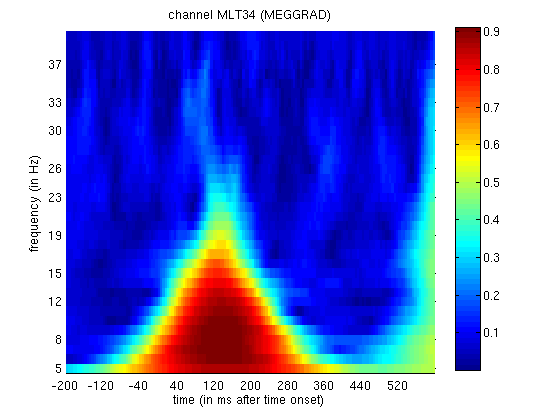
\includegraphics[width=60mm]{multimodal/figures/meg_plv_faces}
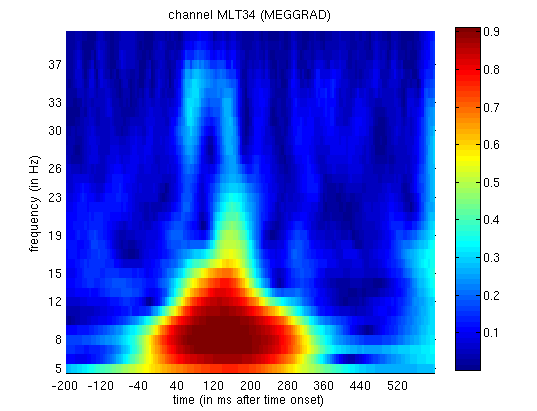
\includegraphics[width=60mm]{multimodal/figures/meg_plv_scrambled}
\caption{\em Phase-Locking Values for faces (left) and scrambled faces (right) for channel MLT34 \label{multimodal:fig:14}}
\end{center}
\end{figure}

\subsection{2D Time-Frequency SPMs}

Analogous to Section~\ref{multimodal:eeg:3DSPM}, we can also use Random Field Theory to correct for multiple statistical comparisons across the 2-dimensional time-frequency space.

Select \textsc{Convert to images} in the ``Other'' pulldown menu, and select the \texttt{tf\_cdbespm8\_\-SPM\_\-CTF\_\-MEG\_\-example\_\-faces1\_\-3D.mat} file. Usually you would be asked whether you want to average over channels or frequencies. In this case there is only one channel in this dataset, so the ``channels'' option will be selected automatically.

This will create 2D time-frequency images for each trial of the two types with dimensions $36\times 161\times 1$, as for the example shown in Figure~\ref{multimodal:fig:15}. These images can be found in the subdirectories \texttt{1ROI\_TF\_\-trialtype\_\-faces} and \texttt{1ROI\_TF\_\-trialtype\_\-scrambled} of the new directory created \texttt{tf\_\-cdbespm8\_\-SPM\_\-CTF\_\-MEG\_\-example\_\-faces1\_3D}, and examined by pressing ``Display: images'' on the main SPM window.

\begin{figure}
\begin{center}
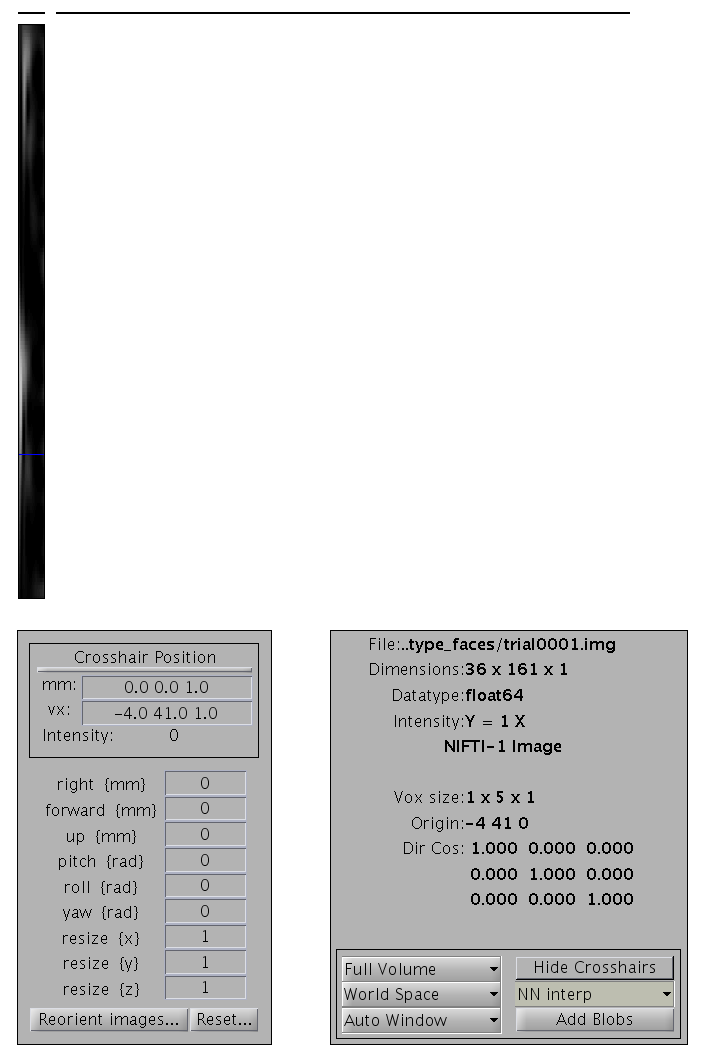
\includegraphics[width=100mm]{multimodal/figures/meg_TFimage}
\caption{\em  3D image for trial 2 within \texttt{1ROI\_TF\_trialtype\_faces} subdirectory. The bottom left section is through frequency (x) and time (y) (the other images are strips because there is only one value in the z dimension, i.e, this is really a 2D image).\label{multimodal:fig:15}}
\end{center}
\end{figure}

As in Section~\ref{multimodal:eeg:3Dsmooth}, these images can be further smoothed in time and frequency if desired. 

Then as in Section~\ref{multimodal:eeg:3DSPM}, we then take these images into an unpaired t-test across trials to compare faces versus scrambled faces. We can then use classical SPM to identify times and frequencies in which a reliable difference occurs, correcting across the multiple comparisons entailed (Kilner et al, 2005).

First create a new directory, eg. \texttt{mkdir TFstatsPow}.

Then press the \textsc{specify 2nd level} button, select ``two-sample t-test'' (unpaired t-test), and define the images for ``group 1'' as all those in the subdirectory \texttt{trialtype\_faces} (using right click, and ``select all'') and the images for ``group 2'' as all those in the subdirectory \texttt{trialtype\_scrambled}. Finally, specify the new \texttt{TFstatsPow} directory as the output directory. (Note that this will be faster if you saved and could load an SPM job file from Section~\ref{multimodal:eeg:3DSPM} in order to just change the input files and output directory.) Then add an ``Estimate'' module from the ``SPM'' tab, and select the output from the previous factorial design specification stage as the dependency input. Press ``Run'' (green arrow button).

Press \textsc{Results} and define a new T-contrast as $[1\: -1]$. Keep the default contrast options, but threshold at $p<.05$ FWE corrected for the whole search volume, and then select ``Time-Frequency'' for the ``Data Type''. Then press ``whole brain'', and the Graphics window should now look like that in Figure~\ref{multimodal:fig:16}.

\begin{figure}
\begin{center}
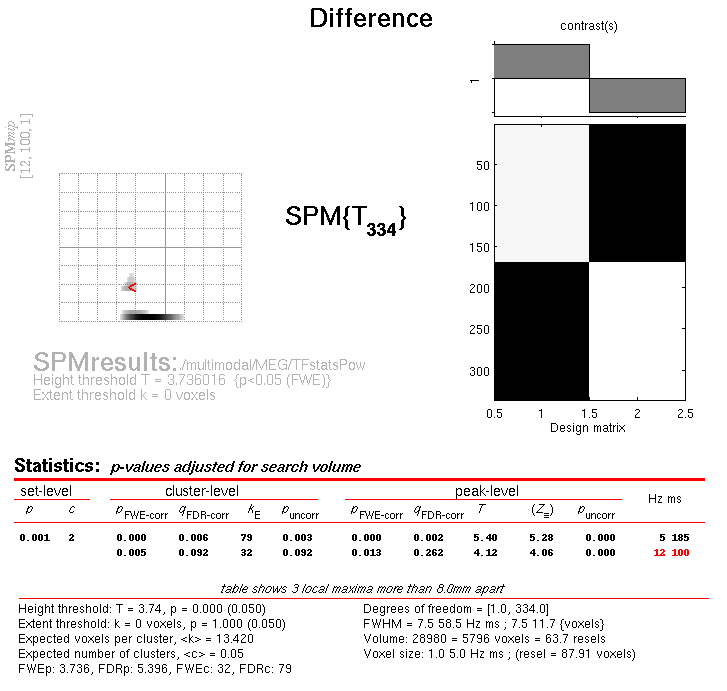
\includegraphics[width=100mm]{multimodal/figures/meg_TF_results}
\caption{\em 2D time-frequency SPM{T} at $p<.05$ FWE-corrected for the power difference between face and scrambled faces at Channel MLT34.\label{multimodal:fig:16}}
\end{center}
\end{figure}

This will list two ``regions'' within the 2D time-frequency space in which faces produce greater power than scrambled faces, having corrected for multiple T-tests across pixels. The larger one has a maximum at 5 Hz and 185 ms post-stimulus, corresponding to the M170 seen earlier in the averaged files (but now with a statistical test of its significance, in terms of evoked and induced power). The second, smaller region has a maximum at 12 Hz and 100 ms, possibly corresponding to a smaller but earlier effect on the M100 (also sometimes reported, depending on what faces are contrasted with).

\subsection{``Imaging'' reconstruction of total power for each condition \label{multimodal:data:meg:recon_pow}}

In Section~\ref{multimodal:eeg:3D} we localised the differential evoked potential difference in EEG data corresponding to the N170.  Here we will localise the total power of faces, and of scrambled faces, ie including potential induced components (see Friston et al, 2006).

Press the ``3D source reconstruction'' button, and press the ``load'' button at the top of the new window. Select the \texttt{cdbespm8\_SPM\_CTF\_MEG\_example\_faces1\_3D.mat} file and type a label (eg \texttt{M170}) for this analysis.

Press the ``MRI'' button, select the \texttt{smri.img} file within the \texttt{sMRI} sub-directory and select the ``normal'' mesh.

If you have not used this MRI image for source reconstruction before, this step will take some time while the MRI is segmented and the deformation parameters computed (see Section~\ref{multimodal:eeg:3D} for more details on these files). When meshing has finished, the cortex (blue), inner skull (red) and scalp (orange) meshes will also be shown in the Graphics window with slices from the sMRI image. This makes it possible to verify that the meshes indeed fit the original image well. The field \texttt{D.inv\{1\}.mesh} will be updated. Press ``save'' in top right of window to update the corresponding mat file on disk.

Both the cortical mesh and the skull and scalp meshes are not created directly from the segmented MRI, but rather are determined from template meshes in MNI space via inverse spatial normalisation (Mattout et al, 2007; Henson et al, 2009a).

Press the ``Co-register'' button. You will be asked for each of the 3 fiducial points to specify its location on the MRI images. This can be done by selecting a corresponding point from a hard-coded list (``select''). These points are inverse transformed for each individual image using the same deformation field that is used to create the meshes. The other two options are typing the MNI coordinates for each point (``type'') or clicking on the corresponding point in the image (``click''). Here, we will type coordinates based on where the experimenter defined the fiducials on the \texttt{smri.img}. These coordinates can be found in the \texttt{smri\_fid.txt} file also provided. So press ``type'' and for ``nas'', enter [0  91  -28]; for ``lpa'' press ``type'' and enter [-72   4  -59]; for ``rpa'' press ``type'' and enter [71  -6  -62]. Finally, answer ``no'' to ``Use headshape points?'' (see EEG Section~\ref{multimodal:eeg:3D}).

This stage coregisters the MEG sensor positions with the structural MRI and cortical mesh, via an approximate matching of the fiducials in the two spaces, followed by a more accurate surface-matching routine that fits the head-shape function (measured by Polhemus) to the scalp that was created in the previous meshing stage via segmentation of the MRI. When coregistration has finished, the field \texttt{D.inv\{1\}.datareg} will be updated. Press ``save'' in top right of window to update the corresponding mat file on disk. With the \matlab\ Rotation tool on (from the ``Tools'' tab in the SPM Graphics window, if not already on), right click near the top image and select ``Go to X-Z'' view. This should produce a figure like that in Figure~\ref{multimodal:fig:17}, which you can rotate with the mouse to check all sensors. Note that the data are in head space (not MNI space), in this case corresponding to the Polhemus space in which the X and Y dimensions are swapped relative to MNI space.

\begin{figure}
\begin{center}
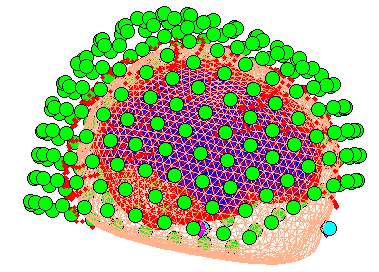
\includegraphics[width=70mm]{multimodal/figures/meg_coreg.png}
\caption{\em  Graphical output of registration of MEG and sMRI data, showing (upper panel) cortex (blue) and scalp (black) meshes, sensor locations (green), MRI and Polhemus fiducials (cyan/magneta), and headshape (red dots).\label{multimodal:fig:17}}
\end{center}
\end{figure}

Press the ``Forward Model'' button. Choose ``MEG Local Spheres'' (you may also try the other options; see Henson et al, 2009a). A figure will be displaying showing the local (overlapping) spheres fit to each sensor, and final the set of all spheres.

Press ``Invert'', select ``Imaging'', select ``yes'' to ``All conditions or trials?'', and ``Standard'' for the model (i.e, to use defaults; you can customise a number of options if you press Custom instead) (see Friston et al, 2008, for more details about these parameters). There will be lead field computation followed by the actual inversion. A summary plot of the results will be displayed at the end.

You can now explore the results via the 3D reconstruction window. If you type 180 into the box in the bottom right (corresponding to the time in ms) and press ``mip'', you should see several ventral temporal hotspots, as in Figure~\ref{multimodal:fig:18}. Note that this localisation is different from the previous EEG localisation because 1) condition 1 now refers to faces, not the difference between faces and scrambled faces, and 2) the results reflect total power (across trials), induced and evoked, rather than purely evoked\footnote{Though in reality, most of the power is low-frequency and evoked}. The timecourses come from the peak voxel (with little evidence of a face/scrambled difference for this particular maximum). The red curve shows the condition currently being shown (corresponding to the ``Condition 1'' toggle bar in the reconstruction window); the grey curve(s) will show all other conditions. If you press the "condition 1" toggle, it will change to Condition 2, which is the total power for scrambled faces, then press ``mip'' again and the display will update (note the colours of the lines have now reversed from before, with red now corresponding to scrambled faces).

\begin{figure}
\begin{center}
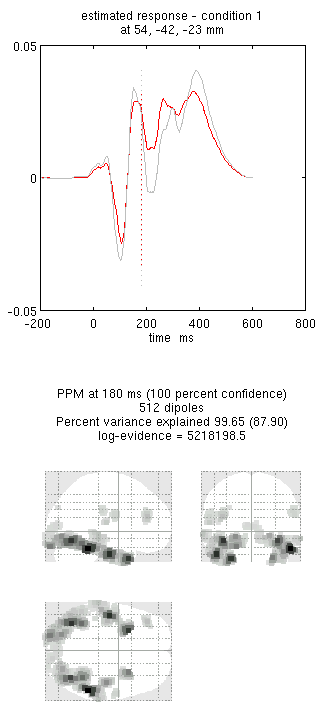
\includegraphics[width=90mm]{multimodal/figures/meg_msp.png}
\caption{\em  Graphic output for MSP-estimated activity at 159ms for faces.\label{multimodal:fig:18}}
\end{center}
\end{figure}


If press ``movie'', you will see the changes in the source strengths over peristimulus time (from the limits 0 to 300ms currently chosen by default).

If you press ``render'' it will open a graphical interface that is very useful to explore the data (the buttons are fairly self-explanatory). 

You can also explore the other inversion options, like COH and IID, which you will note give more superficial solutions (a known problem with standard minimum norm; see also Friston et al, 2008; Henson et al, 2009a). To do this quickly (without repeating the MRI segmentation, coregistration and forward modelling), press the ``new'' button in the reconstruction window, which by default will copy these parts from the previous reconstruction. 

In the following we will concentrate on how one prepares this single subject data for subsequent entry into a group analysis.

Press the ``Window'' button in the reconstruction window, enter ``150 200'' as the timewindow of interest and ``5 15'' as the frequency band of interest (from the SPM time-frequency analysis, at least from one channel). Then choose the ``induced'' option. After a delay (as SPM calculates the power across all trials) the Graphics window will show the mean activity for this time/frequency contrast (for faces alone, assuming the condition toggle is showing ``condition 1'').

If you then press ``Image'', SPM will write 3D NIfTI images corresponding to the above contrast for each condition:

\begin{verbatim}
    cdbespm8_SPM_CTF_MEG_example_faces1_3D_1_t150_200_f5_15_1.nii
    cdbespm8_SPM_CTF_MEG_example_faces1_3D_1_t150_200_f5_15_2.nii
\end{verbatim}

The last number in the file name refers to the condition number; the number following the dataset name refers to the reconstruction number (i.e. the number in red in the reconstruction window, i.e, \texttt{D.val}, here 1).

The smoothed results for Condition 1 will also be displayed in the Graphics window, together with the normalised structural. Note that the solution image is in MNI (normalised) space, because the use of a canonical mesh provides us with a mapping between the cortex mesh in native space and the corresponding MNI space.

You can also of course view the image with the normal SPM ``Display:image'' option, and locate the coordinates of the ``hotspots'' in MNI space. Note that these images contain RMS (unsigned) source estimates (see Henson et al, 2007).

If you want to see where activity (in this time/freq contrast) is greater for faces and scrambled faces, you can use SPM \texttt{ImCalc} facility to create a difference image of \texttt{cdbespm8\_\-SPM\_\-CTF\_\-MEG\_\-example\_\-faces1\_\-3D\_\-1\_\-t150\_\-200\_\-f5\_\-15\_\-1.nii} - \texttt{cdbespm8\_\-SPM\_\-CTF\_\-MEG\_\-example\_\-faces1\_\-3D\_\-1\_\-t150\_\-200\_\-f5\_\-15\_\-2.nii}: you should see bilateral fusiform. For further discussion of localising a differential effect (as in Section~\ref{multimodal:eeg:3D} with ERPs), vs taking the difference of two localisations, as here, see Henson et al (2007). The above images can then be used at the second level (assuming one also has data from other subjects) to look for effects that are consistent over a group of subjects.

